\section{Analysis of the Fault Model}
\label{sec:fault_analysis}
There are two possible fault analyses available to users, monolithic and compositional. 
The purpose of the safety analysis process is to guarantee that certain top level safety properties of the system hold with certain probability in the presence of faults. 

\janet{Janet Note TODO: consider combine the first three subsections and update the last section to talk from users/use case stand point of view - walk through concrete examples to show how we use the analysis capabilities mentioned in the original subsections to help address the problem we raised in the intro/prelim section}
\danielle{Danielle Note: Reading through a paper, I believe it is helpful to have subsections to make the distinction clear. It makes it less of a block of text. Yeah, not super important, but having the subsections makes each topic a little clearer to see. I vote to keep them.}

\subsection{Fault Hypothesis}

An annotation in the AADL model determines the fault hypothesis. This may specify either a maximum number of faults that can be active at any point in execution or that only faults whose probability of simultaneous occurrence is above some probability threshold should be considered (see Figure~\ref{fig:hwFaultProp}). Tying back to traditional safety analysis, the former is analogous to restricting the cutsets to a specified maximum number of terms, and the latter is analogous to restricting the cutsets to only those whose probability is above some set value.

In the former case, we assert that the sum of the true {\em fault\_\_trigger} variables is below some integer threshold.  In the latter, we determine all combinations of faults whose probabilities are above the specified probability threshold, and describe this as a proposition over {\em fault\_\_trigger} variables. 
%
With the introduction of dependent faults, active faults are divided into two categories: independently active (activated by its own triggering event) and dependently active (activated when the faults they depend on become active). The top level fault hypothesis applies to independently active faults. Faulty behaviors augment nominal behaviors whenever their corresponding faults are active (either independently active or dependently active).

\begin{comment}
\subsection{Architecture and Implementation}
\label{sec:implementation}

The architecture of the Safety Annex is shown in Figure~\ref{fig:plugin-arch}.  It is written in Java as a plug-in for the OSATE AADL toolset, which is built on Eclipse.  It is not designed as a stand-alone extension of the language, but works with behavioral contracts specified in AGREE AADL annex and associated tools~\cite{NFM2012:CoGaMiWhLaLu}.  AGREE allows {\em assume-guarantee} behavioral contracts to be added to AADL components.  The language used for contract specification is based on the Lustre dataflow language~\cite{Halbwachs91:IEEE}. AGREE improves scalability of formal verification to large systems by decomposing the analysis of a complex system architecture into a collection of smaller verification tasks that correspond to the structure of the architecture.

\begin{figure}
	\begin{center}
		%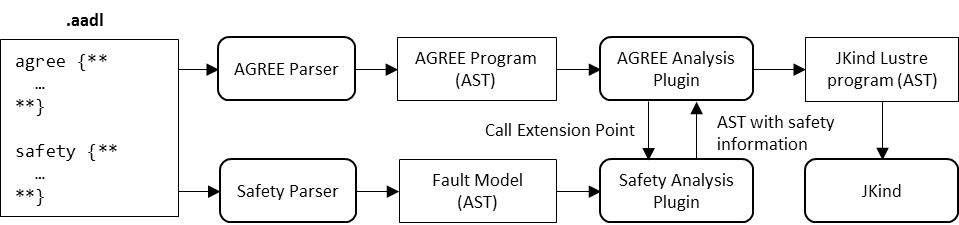
\includegraphics[trim=0 400 430 0,clip,width=0.85\textwidth]{images/arch.png}
		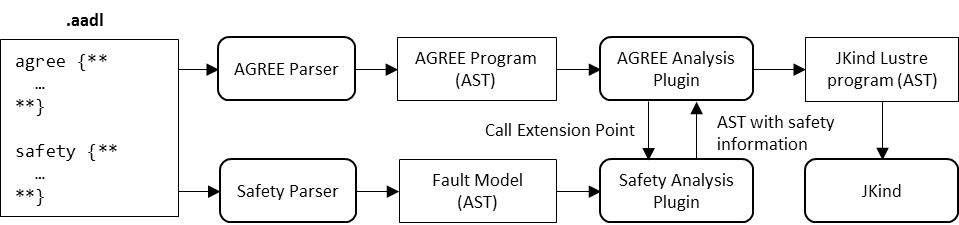
\includegraphics[width=.9\textwidth]{images/arch.png}
	\end{center}
	\vspace{-0.2in}
	\caption{Safety Annex Plug-in Architecture}
	\label{fig:plugin-arch}
\end{figure}

AGREE contracts are used to define the nominal behaviors of system components as {\em guarantees} that hold when {\em assumptions} about the values the component's environment are met.  The Safety Annex extends these contracts to allow faults to modify the behavior of component inputs and outputs.  To support these extensions, AGREE implements an Eclipse extension point interface that allows other plug-ins to modify the generated abstract syntax tree (AST) prior to its submission to the solver.  If the Safety Annex is enabled, these faults are added to the AGREE contract and, when triggered, override the nominal guarantees provided by the component.  

An example of a portion of an initial AGREE node and its extended contract is shown in Figure~\ref{fig:lustre}. 
In the left column of the figure, the nominal Lustre pump definition is shown with an AGREE contract on the output. In the right column, the additional local variables for the fault are seen in boxes 1 and 2, the assertion binding the fault value to the nominal value is seen in boxes 3 and 4, and the fault node definition is given in box 5. 

\begin{figure}[h!]
	\hspace*{-2cm}
	\vspace{-0.3in} 
	\begin{center}
		%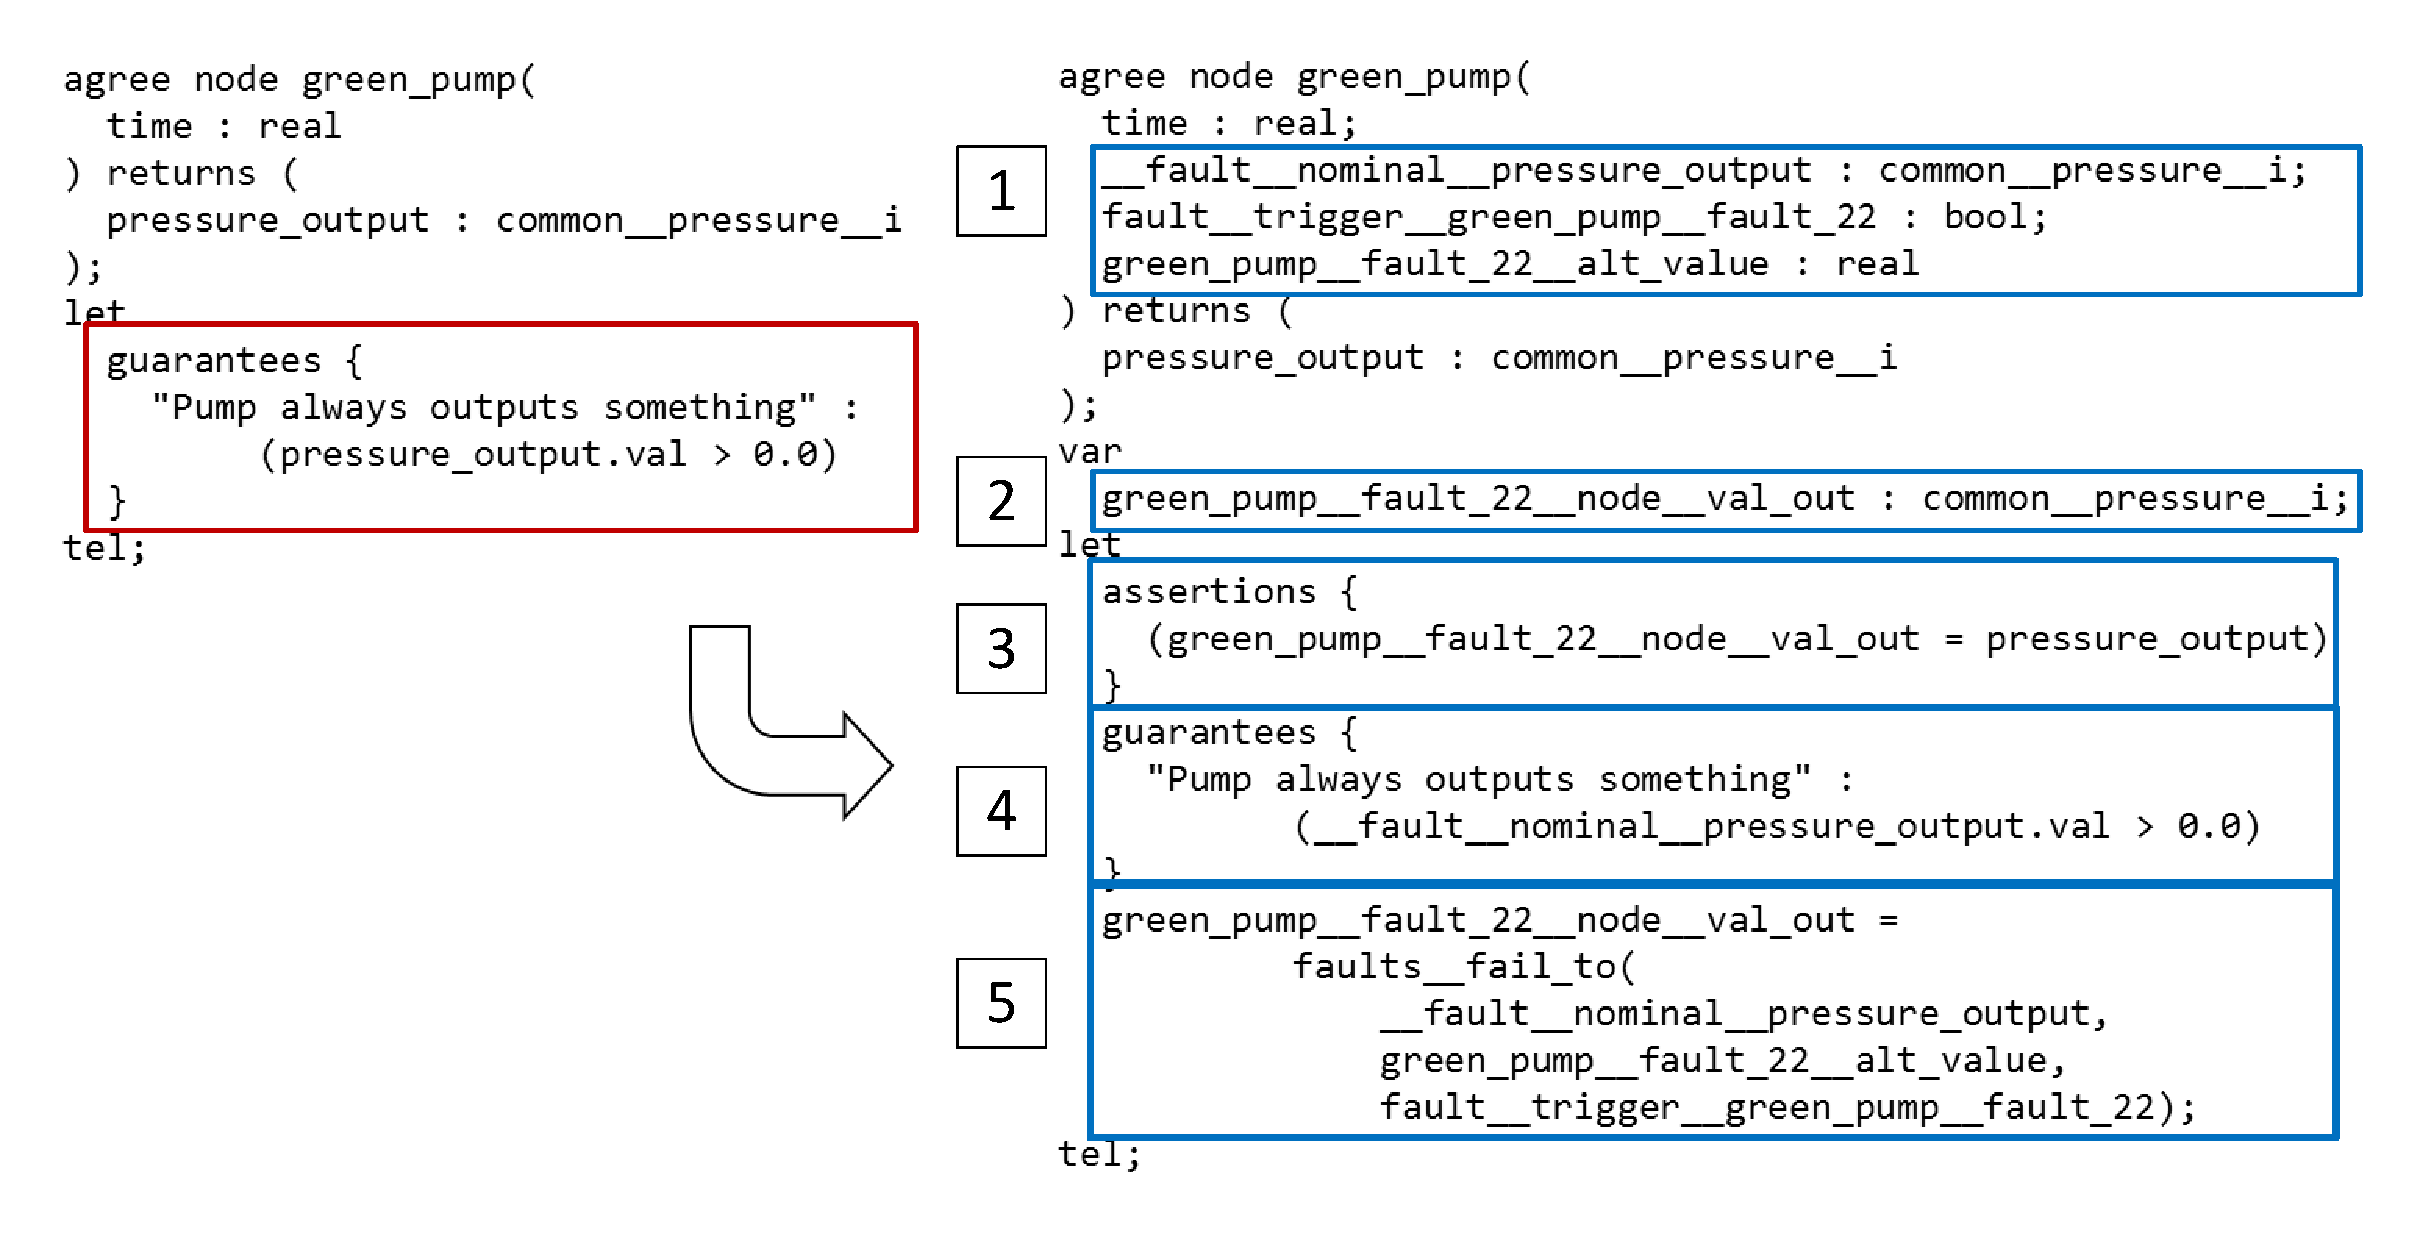
\includegraphics[trim=0 690 -10 70,clip,width=1.5\dimexpr\textwidth-2cm\relax]{images/lustre.pdf}
		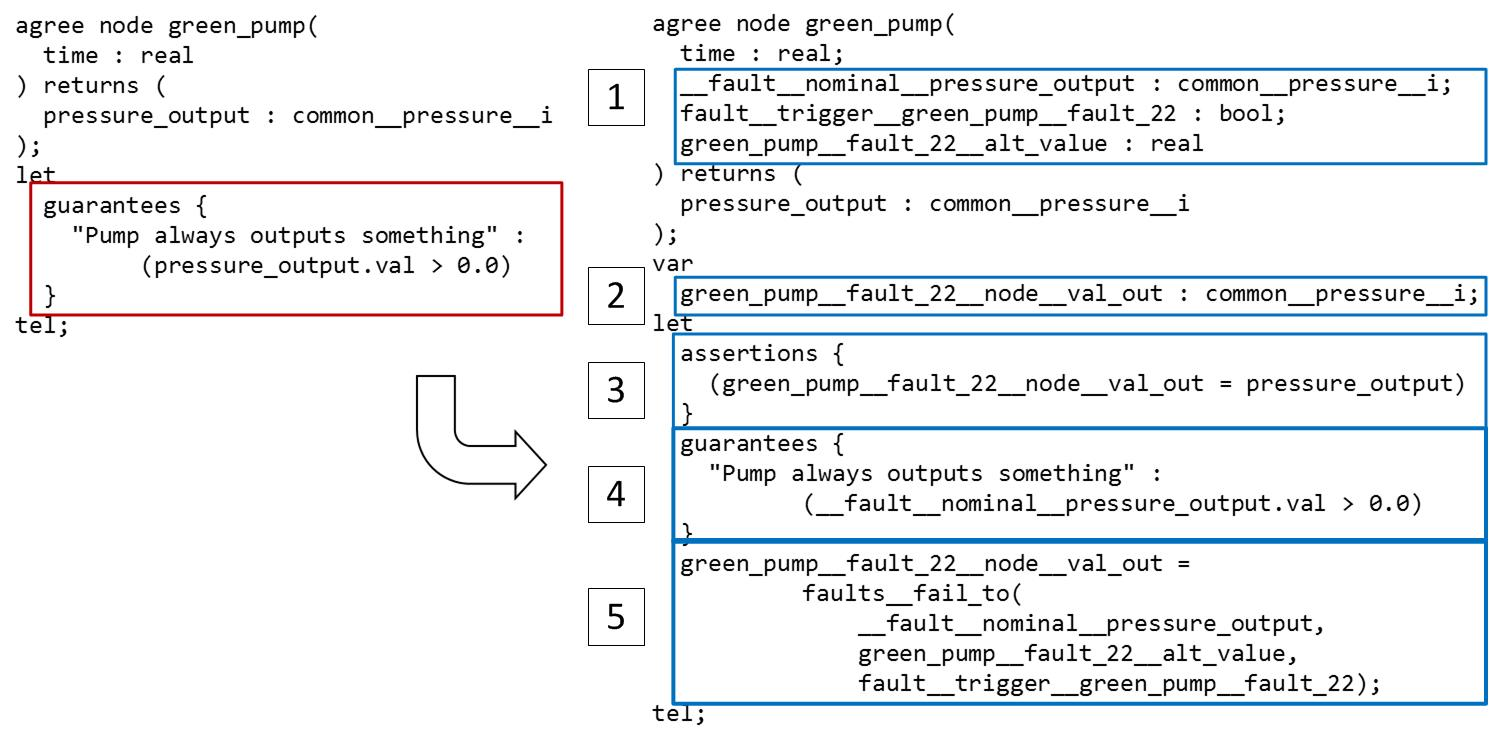
\includegraphics[scale=0.3]{images/lustre.jpg}
		\caption{Nominal AGREE node and its extension with faults}
		\label{fig:lustre}
	\end{center}
	\vspace{-0.3in}
\end{figure}


Once augmented with fault information, the AGREE model follows the standard translation path to the model checker JKind~\cite{2017arXiv171201222G}, an infinite-state model checker for safety properties.  The augmentation includes traceability information so that when counterexamples are displayed to users, the active faults for each component are visualized.

\end{comment}

\subsection{Monolithic Analysis}


When monolithic analysis is performed on the nominal system model, the architectural model is flattened in order to perform the analysis. All of the contracts in the lower levels are used for the analysis.
A top level threshold is defined within the safety annex located in the top level system implementation. In the lower levels, each defined subcomponent fault is given a probability of occurrence. To perform this analysis, it is assumed that the non-hardware faults occur independently and possible combinations of faults are analyzed by the model checker. This corresponds to performing a prior analysis on which combinations of faults have a probability less than the threshold and then inserting assertions into the Lustre code accordingly. If the probability of such combination of faults is in fact less than the designated top level threshold, these faults may be activated and the behavioral effects can be seen through a counterexample.  

\begin{algorithm}[H]
% \KwData{this text}
% \KwResult{how to write algorithm with \LaTeX2e }
 $\mathcal{F} = \{\}$ : fault combinations above threshold \;
 $\mathcal{Q}$ : faults, $q_i$, arranged with probability high to low \;
 $\mathcal{R} = \mathcal{Q}$ , with $r \in \mathcal{R}$\;
 \While{$\mathcal{Q} \neq \{\} \land \mathcal{R} \neq \{\}$ }{
   $q =$ removePriorityElement($\mathcal{Q}$) \;
   \For{$i=0:|\mathcal{R}|$}{
       $prob = q \times r_i$ \;
       \eIf{prob $<$ threshold}{
         removeTail($\mathcal{R}, j=i:|\mathcal{R}|$)\;
       }{
        add($\{q, r_i\}, \mathcal{Q}$)\;
        add($\{q, r_i\}, \mathcal{F}$)\;
      } % end if else
   } % end for
 } % end while
 \caption{Monolithic Probability Analysis}
\end{algorithm}

The algorithm first removes all faults from consideration that are too unlikely given the probability threshold. The remaining faults are arranged in a priority queue $\mathcal{Q}$ from high to low. Assuming independence in the set of faults, we take a fault with highest probability from the queue (step 5) and attempt to combine the remainder of the faults in $\mathcal{R}$ (step 7). If this combination is lower than the threshold (step 8), then we do not take into consideration this set of faults and instead remove the tail of the remaining faults in $\mathcal{R}$. The reason we can do this is because of the arrangement in priority queue from highest to lowest value. If this combination is below threshold, certainly any other combination of these faults with one of lesser value in the priority queue will also be below threshold. 
 
In this calculation, we assume independence among the faults, but in the Safety Annex, it is possible to define dependence between faults using a \textit{hardware fault} node. At the end of Algorithm 1, the possible fault combinations reside in the list $\mathcal{F}$. We then look at the collection of propagation statements used in HW fault definitions. These have a source (HW fault) and destination (faults triggered by HW fault). 

Let $\mathcal{P}$ be the collection of propagation statements. For all $S \subset \mathcal{F}$, check to see if for $f \in S$, $f \in \mathcal{P}$ as a source. If so, add the corresponding destinations to the set $S$. This set $\mathcal{F}$ of allowed fault combinations is then added as a constraint to the Lustre model and thus they become active. If an active fault causes the violation of a contract, this is seen in a counterexample provided by the model checker.

\subsection{Compositional Analysis}
In compositional analysis, the analysis proceeds in a top down fashion. To prove the top level properties, the properties in the layer directly beneath the top level are used to perform the proof. The analysis proceeds in this manner.

 Users can constrain the maximum number of faults within each layer of the model by specifying the maximum fault hypothesis statement to that layer. If any lower level property failed due to activation of faults, the property verification at the higher level can no longer be trusted as the higher level properties were proved based on the facts that its direct sub level properties are valid.
 
For compositional anlaysis, fault hypotheses (see Figure 3) must be added to each layer of a system in order for analysis to proceed correctly. Also, at most one of the analysis statements must be present. 
 
 This type of analysis is helpful to see weaknesses in a given component or layer of the system. In future work, we plan to reflect lower level property violations in the verification results of higher layers in the architecture, and enable displaying or constraining active faults system wide instead of component wide.

\subsection{Analysis Results of the WBS Example}
\label{sec:results}

Fault analysis on the top level WBS system was performed on the 11 top-level properties using two fault hypotheses.  In the first case, we allow at most one fault, and in the second we allow combinations of faults that exceed the acceptable probability for the top-level hazard defined in AIR6110.

We use this model to demonstrate the benefits of formal fault analysis and to show the scalability of our tools.  We applied both monolithic and compositional analysis.

\janet{Janet Note: TODO: replace timing data on something about what we learned from the analysis results, and use it to feedback to the system design, and rerun the analysis. As Mats pointed out, "can we add a redundant sensor and get fault tolerance?}
\danielle{Danielle Note: The last 2 paragraphs of this section addresses this idea a little bit. One thing we can do is add a redundant sensor to the wbs model and run it to see what happens. If we do not want to add more to the model and perform analysis, then perhaps the last paragraphs of this section is good enough.}

%For the fault-free ``nominal'' system model, monolithic analysis requires 21 seconds, whereas compositional analysis requires 1 minute and 53 seconds.  Although the compositional time is longer, each sub-problem completes in less than 5 seconds.  The additional time for compositional analysis is  due to the start-up overhead to invoke the JKind model checker many times for individual layers.  On the other hand, when examining the model under a single-fault hypothesis, compositional analysis requires 2 minutes 6 seconds, while monolithic analysis did not terminate after 60 minutes.

%For probabilistic fault hypotheses, we are currently developing a sound approach for composition with respect to the top-level fault probability, but our current tool requires monolithic analysis.  In this case, given a probabilistic fault hypothesis of $5\times 10^{-7}$, monolithic analysis requires 3 minutes 25 seconds.

During our analysis, we discovered that most properties were verified, but the \textit{Inadvertent braking at the wheel} properties are not resilient to a single fault nor do they meet the desired $10^{-9}$ fault threshold for probabilistic analysis.  In this model, there is a single pedal position sensor for the brake pedal.  If this sensor fails, it can command braking without a pilot request.  Given the {\em counterexample} returned by the tools, it is straightforward to diagnose the fault conditions that lead to property failure.

This counterexample can be used to further analyze the system design.  For our model, there are several possible reasons for failure: it could be that redundant sensors are required on the pedals (here we note that the architecture of the pedal assembly is not discussed in AIR6110) or that the phase of flight is sufficiently short that we need to adjust our pedal failure rate to match this phase of flight, rather than normalizing the failure rate to per-flight-hour.  

It is computationally inexpensive to run the analysis, allowing quick iterations between systems and safety engineers. 
In the case of the WBS, it requires between 2 and 4 minutes to run either compositional (restricting the number of faults) or monolithic (probabilistic) fault analysis on the model.
The sync and update between the safety analysis artifacts and the system architecture/analysis model continues until the system safety property is satisfied with the desired fault tolerance and failure probability achieved.